\section{Efficient Enumeration of Laddder Lotteries and its Application}
In their paper, Efficient Enumeration of Ladder Lotteries and its Application,
the authors provide an algorithm for generating $OptL\{\pi\}$ 
for any $\pi$, in $\mathcal{O}(1)$ per ladder \cite{A1}. This is the first and only 
published algroithm for generating $OptL\{\pi\}$. The paper also presents the number 
of ladder lotteries in $OptL\{(11, 10, 9, 8, 7, 6, 5, 4, 3, 2, 1)\}$ which is 
$5,449,192,389,984$ \cite{A1}. This is a very impressive accomplishment for reasons which 
will be discussed later in the literature review.\par 
The authors' algorithm is based on several key concepts, the most 
important of which is the \emph{local swap operation}. This is the 
minimal change operation that transitions from one ladder in $OptL\{\pi\}$ to the 
next ladder. The local swap operation is essentially a 180 degree rotation
of three bars in the ladder, such that the bottom
bar is rotated to the top, the middle bar stays in the middle and the top bar
is rotated to the bottom. If the bars undergo a 180 degree rotation to the right, 
then this is known as a \emph{right swap operation} and 
if the bars udergo a 180 degree rotation to the left then this 
is known as a \emph{left swap operation}. To go to the next ladder in the set, 
the current ladder, $L_{i}$ udergoes a right swap operation 
to get to ladder $L_{i+1}$. See Fig. 2.2 for an exmaple of a 
local swap operation.The \emph{route} of an element is the sequence of bars in the ladder that an element must cross in order to reach its correct position in 
the identity permutation. The sequence is ordered from top left to bottom right.
Note that each bar has two elements that cross it, 
therefore the bar belongs to the route of the greater of the two elements. 
It is important to note that when a right swap operation occurs, 
two of the three bars belong to the route of a greter element and one bar belongs
to the route of a lesser element. Once rotated, the bar of the lesser element is 
above the bars of the greater element.\par
The \emph{clean level} refers to the smallest element 
in $\pi$ such that none of its bars have undergone a right swap operation.
If there is no such element, then the clean level is the maximum element in $\pi$ + 1.
The \emph{root ladder} is the only ladder in  the set with a clean level of 1; in 
other words, the root ladder is the only ladder in which no bars have undergone 
a right swap operation. The root ladder is unique to $OptL\{\pi\}$. To see the root ladder 
of $OptL\{(4,5,6,3,1,2)\}$ please refer to figure Fig. 2.3. Since none of
the bars in the root ladder have undergone a right swap operation, it is the only 
ladder in $OptL\{\pi\}$ that has a clean level of $1$. The root ladder is
also the original decendant ladder in the set. Insofar as the enumeration algorithm 
is based on performing a right swap operation on a pervious ladder, then every other 
ladder must have at least one right swap operation. Since the root ladder has
no right swap operations, then it must be the decendant of every other ladder.\par 
The algorithm for generating $OptL\{\pi\}$ in the paper was the backbone 
of the research for this thesis. However, the algorithm in this paper had some 
issues. These issues presented several challenges during the research for this thesis.
The first issue in the paper is that the authors do not provide an algorithm for
generating the root ladder in $OptL\{\pi\}$. Seeing as every other in the set 
is derived from the root ladder, it is essential to build the root ladder without
performing a right swap operation. Yet the paper does not provide such an 
algorithm. The second issue in this paper is that there is no algorithm 
for permforming a local swap operation on a ladder. Although the authors 
do a good job explaining under what conditions a local swap operation can 
be performed \cite{A1}, the actual operation itself is trickier than it seems. The last 
issue in the paper is that it contains an error. The error is that one of the diagrams is incorrect. 
The diagram is of all the ladders in $OptL\{(5,6,3,4,2,1)\}$. This diagram contains 76 
ladders when there are actually only 75. The error was confirmed by the author Yamanaka in an 
email correspondence he and I had. These issues will be resolved in the Methodology and Implementation
section.
%%If the root ladder is the ladder generated by the SJT algorithm for all permutations
%%of size N, then emphasize that the solution the the Gray Code is that the ladders 
%generated are root ladders. 
%%write a proof for the terminating ladder, which shows that it is unique and is the 
%%only ladder in the set in which no left swap operation is possible in the methods section
%%when you go over how the algorithm works

\begin{figure}[!htp]
	\begin{minipage}{0.4\textwidth}
		\begin{center}

			%%drawing the lines
			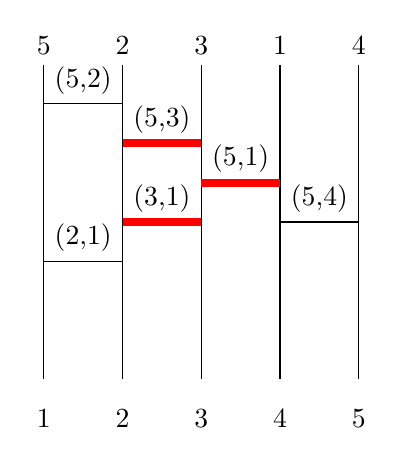
\begin{tikzpicture}
				\draw(0, 0) to (0, 4) node[above]{5};
				\node at (0, -0.5){1};

				\draw(1, 0) to (1, 4) node[above]{2};
				\node at (1, -0.5){2};


				\draw(2, 0) to (2, 4) node[above]{3};
				\node at (2, -0.5){3};

				\draw(3, 0) to (3, 4) node[above]{1};
				\node at (3, -0.5){4};


				\draw(4, 0) to (4, 4) node[above]{4};
				\node at (4, -0.5){5};

				%%drawing the bars

				%%5's route
				\draw(0, 3.5)to (1, 3.5);
					\draw node at (0.5, 3.8) {(5,2)};
				\draw[line width=1mm, red](1, 3) to (2, 3);
					\draw node at (1.5, 3.3) {(5,3)};
				\draw[line width=1mm, red](2, 2.5) to (3, 2.5);
					\draw node at (2.5, 2.8) {(5,1)};
				\draw(3, 2) to (4, 2);
					\draw node at (3.5, 2.3) {(5,4)};

				%%4's route, no bars

				%%3s route
				\draw[line width=1mm, red](1, 2) to (2, 2);
					\draw node at (1.5, 2.3) {(3,1)};
				%%2s route
				\draw(0, 1.5) to (1, 1.5);
					\draw node at (0.5, 1.8){(2,1)};
			\end{tikzpicture}
		\end{center}
	\end{minipage}
	\begin{minipage}{0.4\textwidth}
		\begin{flushright}

			%%drawing the lines
			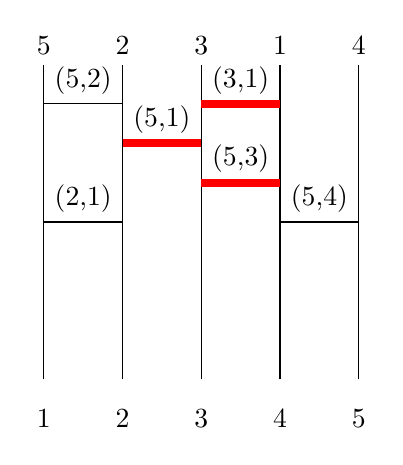
\begin{tikzpicture}
				\draw(0, 0) to (0, 4) node[above]{5};
				\node at (0, -0.5){1};

				\draw(1, 0) to (1, 4) node[above]{2};
				\node at (1, -0.5){2};


				\draw(2, 0) to (2, 4) node[above]{3};
				\node at (2, -0.5){3};

				\draw(3, 0) to (3, 4) node[above]{1};
				\node at (3, -0.5){4};


				\draw(4, 0) to (4, 4) node[above]{4};
				\node at (4, -0.5){5};

				%%Drawing the bars
				\draw(0, 3.5)to (1, 3.5);
					\draw node at (0.5, 3.8){(5,2)};
				\draw[line width=1mm, red](2, 3.5) to (3, 3.5);
					\draw node at (2.5, 3.8) {(3,1)};
				\draw[line width=1mm, red](2, 2.5) to (3, 2.5);
					\draw node at (2.5, 2.8) {(5,3)};
				\draw(3, 2) to (4, 2);
					\draw node at (3.5, 2.3){(5,4)};
				%%4's route, no bars

				%%3s route
				\draw[line width=1mm, red](1, 3) to (2, 3);
					\draw node at (1.5, 3.3) {(5,1)};
				%%2s route
				\draw(0, 2) to (1, 2);
					\draw node at(0.5, 2.3){(2,1)};
			\end{tikzpicture}
		\end{flushright}
	\end{minipage}
	\caption{Example of a local swap operation. When a right swap operation is permformed
	on the left ladder, the result is the right ladder. When a left swap operation is permformed
	on the right ladder, the result is the left ladder.}
	\label{fig:rightSwap}
\end{figure}


\begin{figure}


	\begin{center}
		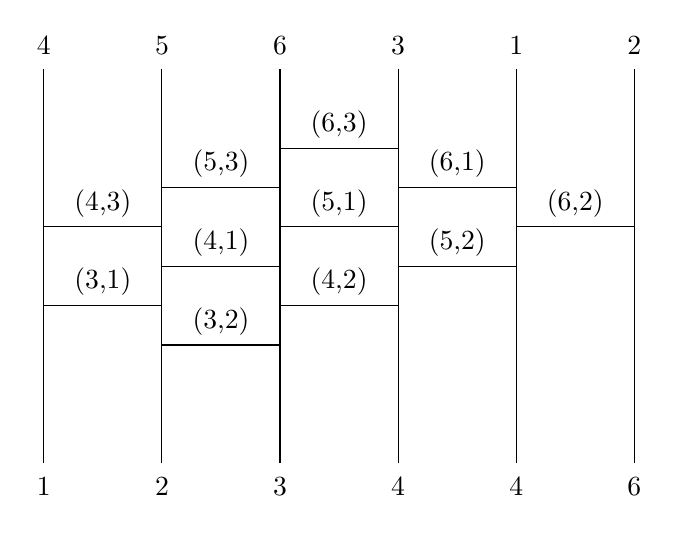
\begin{tikzpicture}
			%%draw the lines
			\draw(0, 0) to (0, 5);
				\node at (0, 5.3){4};
				\node at (0, -0.3){1};

			\draw(1.5, 0) to (1.5, 5);
				\node at (1.5, 5.3){5};
				\node at (1.5, -0.3){2};
			
			\draw(3, 0) to (3, 5);
				\node at (3, 5.3){6};
				\node at (3, -0.3){3};
			\draw(4.5, 0) to (4.5, 5);
				\node at (4.5, 5.3){3};
				\node at (4.5, -0.3){4};
			\draw(6, 0) to (6, 5);
				\node at (6, 5.3){1};
				\node at (6, -0.3){4};
			\draw(7.5, 0) to (7.5, 5);
				\node at (7.5, 5.3){2};
				\node at (7.5, -0.3){6};

			%%draw the bars
			
			%%6's route
			\draw(3, 4) to (4.5, 4);
				\node at (3.75, 4.3){(6,3)};
			\draw(4.5, 3.5) to (6, 3.5);
				\node at (5.25, 3.8){(6,1)};
			\draw(6, 3) to (7.5, 3);
				\node at (6.75, 3.3){(6,2)};
			%%5's route
			\draw(1.5, 3.5) to (3, 3.5);
				\node at (2.25, 3.8){(5,3)};
			\draw(3, 3) to (4.5, 3);
				\node at (3.75, 3.3){(5,1)};
			\draw(4.5, 2.5) to (6, 2.5);
				\node at (5.25, 2.8){(5,2)};
			%draw 4's route
			\draw(0, 3) to (1.5, 3);
				\node at (0.75, 3.3){(4,3)};
			\draw(1.5, 2.5) to (3, 2.5);
				\node at (2.25, 2.8){(4,1)};
			\draw(3, 2) to (4.5, 2);
				\node at (3.75,2.3){(4,2)};

			%%draw 3's route
			\draw(0, 2) to (1.5, 2);
				\node at (0.75, 2.3){(3,1)};
			\draw(1.5, 1.5) to (3, 1.5);
				\node at (2.25, 1.8){(3,2)};
		\end{tikzpicture}

	\end{center}





	\caption{The root ladder for $OptL\{(4,5,6,3,1,2)\}$. Notice how 
	none of the bars have undergone a right swap operation. This is clear 
	when considering that there is no bar of a lesser element above the bar(s)
	of a greater element.} 
	\label{root}

\end{figure}


